\documentclass[a4paper,12pt]{article}

%	---------------------------------	%
%				Titelseite				%
%	---------------------------------	%

% in die entsprechenden Variablen den Inhalt für die Titelseite eintragen

\newcommand{\Studiengang}{Master Informatik
	 
	Modul: Hardware cyber-physischer Systeme}
\newcommand{\Dokumentenart}{Dokumentation}
\newcommand{\Dokumententitel}{Technische Dokumentation Smarte Küchenwaage}
\newcommand{\Autorenname}{Eric Gendner}
\newcommand{\Abgabedatum}{\today}
\newcommand{\Betreuer}{Prof. Dr. Matthias Mörz}

% Variablen für Titelseite des Praxisbericht

\newcommand{\DatumBeginn}{15.03.2022}
\newcommand{\DatumEnde}{\Abgabedatum}
\newcommand{\DatumAbgabe}{\Abgabedatum}

%	---------------------------------	%
%		allgemeine Einstellungen			%
%	---------------------------------	%

%	---------------------------------	%
%		Layout Einstellungen				%
%	---------------------------------	%

% Umlaute unter UTF8 nutzen
\usepackage[utf8]{inputenc}

% deutsche Sonderzeichen und Silbentrennung
\usepackage[ngerman]{babel, translator}

%  Schriftart Times
\usepackage{mathptmx}
\usepackage[scaled=.90]{helvet}
\usepackage{courier}

% Zeichenencoding
\usepackage[T1]{fontenc}
\usepackage{fix-cm}


% Paket für Seitenrandabstände und Einstellung für Seitenränder
\usepackage{geometry}
\geometry{
	left=2.5cm,
	right=2.5cm, 
	top=2.5cm, 
	bottom=3cm
}

% Paragraph styles
\setlength{\parindent}{0cm}
\setlength{\parskip}{6pt}

% Schaltet den zusätzlichen Zwischenraum ab, den LaTeX normalerweise nach einem Satzzeichen einfügt.
\frenchspacing

% Gliederungstiefe einstellen
\setcounter{secnumdepth}{5}
\setcounter{tocdepth}{5}

 
% Kopf- und Fußzeile %

\usepackage{fancyhdr} %Paket laden
\pagestyle{fancy} %eigener Seitenstil
\fancyhf{} %alle Kopf- und Fußzeilenfelder bereinigen
\fancyhead[L]{\nouppercase{\leftmark}} %Kopfzeile links
\fancyhead[C]{} %zentrierte Kopfzeile
\fancyhead[R]{} %Kopfzeile rechts
\renewcommand{\headrulewidth}{0.5pt} %obere Trennlinie
\fancyfoot[R]{\thepage} %Seitennummer
\fancypagestyle{plain}{}
%\renewcommand{\footrulewidth}{0.4pt} %untere Trennlinie

% Abstand Kopf- und Fußzeile vom Rand
\setlength{\headheight}{1.25cm}
\setlength{\footskip}{1cm}

% Abstand Text zur Kopfzeile
\setlength{\headsep}{1cm}


% bricht lange URLs "schoen" um
\usepackage[hyphens,obeyspaces,spaces]{url}

% erzeugt Inhaltsverzeichnis mit Querverweisen zu den Kapiteln (PDF Version)



% Disable single lines at the start of a paragraph (Schusterjungen)
\clubpenalty = 10000

% Disable single lines at the end of a paragraph (Hurenkinder)
\widowpenalty = 10000
\displaywidowpenalty = 10000

% zum Anzeigen des Seitenlayouts
%\usepackage{showframe}


%	---------------------------------	%
%				Pakete					%
%	---------------------------------	%

\usepackage{graphicx}% Grafiken aus PNG Dateien einbinden
\usepackage[onehalfspacing]{setspace}%-- Zeilenabstand 1,5
\usepackage{colortbl}%Einfärben von Tabellen-Zellen, Zeilen, Spalten
\usepackage{tocloft}% Abbildungs- und Tabellenbeschriftung ändern
\usepackage{array}% für Tabellen
\usepackage{multicol}% Paket für multirow Befehl (Tabellen)
\usepackage{multirow}% Paket für multirow Befehl (Tabellen)
\usepackage{longtable}% mehrseitige Tabellen ermöglichen
\usepackage{floatflt}% floatende Bilder ermöglichen
\usepackage{float}
\usepackage{amsmath}% Mathematik Paket
\usepackage{amssymb}% Mathematische Symbole importieren
\usepackage{amsthm}
\usepackage{amsbsy}
\usepackage{textcomp}
\usepackage{upgreek}
\usepackage{wrapfig}
\usepackage{subcaption}
\usepackage{pdfpages}% einbinden von PDF-Dateien
\usepackage{lastpage}
\usepackage{caption}% Paket für Beschriftungen
%\usepackage{ulem}% doppelt unterstreichen \uuline
\usepackage[normalem]{ulem}% doppelt unterstreichen \uuline
\usepackage{tabularx}
\usepackage{lscape}
\usepackage{xcolor}
\usepackage{siunitx}% Paket für SI-Einheiten
\usepackage[right]{eurosym}% Eurozeichen einbinden
\usepackage{color}% Paket für Textfarben
\usepackage{fancybox}% Paket für Boxen im Text
\usepackage{setspace}% Paket für Zeilenabstand
\usepackage{capt-of}% Bildbezeichner
\usepackage[autostyle=true,german=quotes]{csquotes}% Paket für Anführungszeichen
\sisetup{locale = DE}
%\usepackage{hyperref}% Paket für Referenzen
\usepackage[
   colorlinks,        % Links ohne Umrandungen in zu wählender Farbe
   linkcolor=black,   % Farbe interner Verweise
   filecolor=black,   % Farbe externer Verweise
   citecolor=black    % Farbe von Zitaten
]{hyperref}
\usepackage{makeidx}% Stichwortverzeichnis
\usepackage{nomencl}% Symbolverzeichnis
\makenomenclature

%	---------------------------------	%
%			Tabellen und Bilder			%
%	---------------------------------	%

% Rahmen in Textbreite um Objekte
\floatstyle{boxed}
\restylefloat{figure} % Abbildungen
%\restylefloat{table} % Tabellen
\restylefloat{listing} % Codebeispiele

% Captions linksbündig orientieren
\captionsetup{justification=raggedright,singlelinecheck=false}

% Anpassungen Tabellenspalten
% bei fester Ausrichtung Spaltenbreite vorgeben
\newcolumntype{L}[1]{>{\raggedright\arraybackslash}p{#1}}
\newcolumntype{C}[1]{>{\centering\arraybackslash}p{#1}}
\newcolumntype{R}[1]{>{\raggedleft\arraybackslash}p{#1}}

% Anpassung der Tabellenspaltenhöhe
\renewcommand{\arraystretch}{1.2}

% Anpassen der captions
\addto{\captionsngerman}{
\renewcommand*{\figurename}{Abb.}
\renewcommand*{\tablename}{Tab.}
}

% Anpassen der Nummerierung
\numberwithin{equation}{section}

% Tabellenfarben

% Farbdefinitione
%\definecolor{dunkelgrau}{rgb}{0.8,0.8,0.8}
%\definecolor{hellgrau}{rgb}{0.95,0.95,0.95}

%	---------------------------------	%
%			 Codeverzeichnis				%
%	---------------------------------	%

\usepackage{listings}% Paket für Codebeispiele

\lstset{
language=Matlab,
basicstyle=\small\ttfamily\color{black},
commentstyle = \ttfamily\color{green},
keywordstyle=\ttfamily\color{blue},
stringstyle=\color{orange},
backgroundcolor=\color{white},
frame=single,
showstringspaces=false,
captionpos=b,
}

\makeatletter
\begingroup\let\newcounter\@gobble\let\setcounter\@gobbletwo
  \globaldefs\@ne \let\c@loldepth\@ne
  \newlistof{listings}{lol}{\lstlistlistingname}
\endgroup
\let\l@lstlisting\l@listings
\makeatother

\setlength{\cftlistingsindent}{0cm}
\renewcommand*{\cftlistingspresnum}{\lstlistingname~}
\settowidth{\cftlistingsnumwidth}{\cftlistingspresnum}
\addtolength{\cftlistingsnumwidth}{2cm}
\renewcommand{\cftlistingsaftersnum}{:}

% Anpassen der captions
\addto{\captionsngerman}{
\renewcommand*{\lstlistingname}{Code}
}

%	---------------------------------	%
%		Glossar & Symbolverzeichnis		%
%	---------------------------------	%

% Symbolverzeichnis
\newcommand{\nomunit}[1]{%
\renewcommand{\nomentryend}{\hspace*{\fill}#1}}

% Glossar
\usepackage[toc,nonumberlist,acronyms,shortcuts,translate=babel]{glossaries}
\renewcommand*{\glspostdescription}{}
\makeglossaries
\loadglsentries{Dateien/Verzeichnisse/Glossar.tex}



%	---------------------------------	%
%		Literaturverzeichnis				%
%	---------------------------------	%

% Erscheinungsbild
\bibliographystyle{alphadin}


%	---------------------------------	%
%			Abkürzungsverzeichnis		%
%	---------------------------------	%

% Abkürzungen hier eintragen


\newacronym{BLE}{BLE}{Bluetooth Low Energy}
% Indexerstellung
%\makeindex

%	---------------------------------	%
%			Beginn des Dokuments			%
%	---------------------------------	%

\begin{document}

% Symbolverzeichnis
\nomenclature[01]{\textbf{Symbol}}{\textbf{Bedeutung} \nomunit{\textbf{[phys. Einheit]}}}

% Symbole hier eintragen

\nomenclature{$i$}{ganzzahlige Laufvariable}
\nomenclature{$n$}{Umfang der Messreihe oder Stichprobe}
\nomenclature{$s$}{empirische Standardabweichung
	\nomunit{[\si{\metre}]}}
\nomenclature{$\overline{x}$}{Mittelwert der Stichprobe	
	\nomunit{[\si{\metre}]}}
\nomenclature{$x_i$}{Einzelmesswert
	\nomunit{[\si{\metre}]}}

% Worttrennungen
%hier müssen alle Wörter rein, welche Latex von sich aus nicht korrekt trennt bzw. bei denen man die genaue Trennung vorgeben möchte
\hyphenation{
Film-pro-du-zen-ten
Lux-em-burg
Soft-ware-bau-stein
zeit-in-ten-siv
Ab-kürz-ungs-ver-zeich-nis
}

% Titelseite auswählen
%\newgeometry{left=2.5cm, right=2.5cm, top=2.5cm, bottom=2.5cm}

\begin{titlepage}
    \begin{center}
    
\includegraphics[width=\textwidth]{Bilder/Titelseite/Logo_HS_Coburg}
        \begin{Large}
        Hochschule für angewandte Wissenschaften Coburg
        \\
        Fakultät Elektrotechnik und Informatik
        \par
        \end{Large}
        \vspace{1.5cm}
        
        \begin{Large}
            Studiengang: \Studiengang
            \par
        \end{Large}
        \vspace{1.5cm}
        
        \begin{Large}
        	\Dokumentenart
        \end{Large}
        \vspace{1cm}
        
        \begin{Huge}
        	\textbf{\Dokumententitel}
        \end{Huge}
        
        \vspace{2cm}
        
        \begin{huge}
        	\Autorenname
        \end{huge}
        \vspace{2cm}
        
        \begin{Large}
        	Abgabe der Arbeit: \Abgabedatum
        \end{Large}
        
        \begin{Large}
        	Betreut durch:
        \end{Large}
        
        \begin{Large}
        	\Betreuer , Hochschule Coburg
        \end{Large}
        
	\end{center}
    
\end{titlepage}

\restoregeometry
\newgeometry{left=2.5cm, right=2.5cm, top=2.5cm, bottom=2.5cm}

\begin{titlepage}

\begin{center}

\includegraphics[width=\textwidth]{Bilder/Titelseite/Logo_HS_Coburg}

\begin{Large}
	Hochschule für angewandte Wissenschaften Coburg\\
	Fakultät Elektrotechnik und Informatik
	\par
\end{Large}

\vspace{1.5cm}
        
\begin{Large}
	Studiengang: \Studiengang
\par
\end{Large}

\vspace{1.5cm}
        
\begin{Large}
	\Dokumententitel
	
	Betreut durch: \Betreuer
\end{Large}

\vspace{1cm}
        
\begin{huge}
	\Autorenname
\end{huge}

\vspace{1.5cm}   

%\begin{table}[hp]
%	\centering
%	\begin{tabular}{| L{3cm} | L{11cm} |}
%	\hline
%	Unternehmen & \UnternehmenName \\
%	& \UnternehmenAbteilung \\
%	& \UnternehmenStrasse \\
 %	& \UnternehmenOrt \\
%	\hline
%	Zeitraum & \DatumBeginn \ bis \DatumEnde \\
%	\hline
%	\end{tabular}
%\end{table}

\begin{large}
	Abgabe des Berichts: \Abgabedatum
\end{large}

%\begin{table}[hp]
%	\centering
%	\begin{tabular}{| L{3cm} | L{6cm} | L{5cm} |%}
%	\multicolumn{3}{l}{Freigabe zur Vorlage des Praxisberichts an der HS Coburg:} \\
%	\hline
%	Betreuer & \UnternehmenBetreuer & \\
%	\hline
%	Funktion & \BetreuerFunktion & \textbf{\textit{Ort, Datum}}\\
%	\hline
%	Telefon	& \BetreuerTelefon & \\
%	\cline{1-2}
%	email & \BetreuerEmail & \\
%	\hline
 %	& & \textbf{\textit{Unterschrift Betreuer}}\\
%	\hline
%	\end{tabular}
%\end{table}
        
\end{center}
    
\end{titlepage}

\restoregeometry

% Inhaltsverzeichnis
\newpage
\fancyhead[L]{Inhaltsverzeichnis}
\tableofcontents

% Abbildungsverzeichnis
\newpage
\addcontentsline{toc}{section}{Abbildungsverzeichnis}
\fancyhead[L]{Abbildungsverzeichnis}
\renewcommand{\cftfigpresnum}{Abb. }
\renewcommand{\cftfigaftersnum}{:}
\setlength{\cftfignumwidth}{2cm}
\setlength{\cftfigindent}{0cm}
\listoffigures

% Tabellenverzeichnis
\newpage
\addcontentsline{toc}{section}{Tabellenverzeichnis}
\fancyhead[L]{Tabellenverzeichnis}
\renewcommand{\cfttabpresnum}{Tab. }
\renewcommand{\cfttabaftersnum}{:}
\setlength{\cfttabnumwidth}{2cm}
\setlength{\cfttabindent}{0cm}
%\listoftables


% Codebeispielverzeichnis
\newpage
\addcontentsline{toc}{section}{Codebeispielverzeichnis}
\fancyhead[L]{Codebeispielverzeichnis}
%\renewcommand{\lstlistlistingname}{Codebeispielverzeichnis}
%\lstlistoflistings

% Symbolverzeichnis
\newpage
\addcontentsline{toc}{section}{Symbolverzeichnis}
\fancyhead[L]{Symbolverzeichnis}
\renewcommand{\nomname}{Symbolverzeichnis}
\printnomenclature[1in]

% Abkürzungsverzeichnis
\newpage
\fancyhead[L]{Abkürzungsverzeichnis}
%\setglossarystyle{super}
%\printglossary[type=\acronymtype,title=Abkürzungsverzeichnis]

\newpage
\fancyhead[L]{\nouppercase{\leftmark}}

%	---------------------------------	%
%			 	Inhalt					%
%	---------------------------------	%


\section{Einleitung\label{Kap.:Einleitung}}

Die analoge Welt wird immer digitaler, mit dem Einzug der Mikroelektronik wurden analoge Messvorrichtungen durch meist präzisere, digitale Sensoren ersetzt. Dieses Konzept zieht sich durch alle Bereiche des Lebens. Mit dem Aufkommen und der starken Verbreitung von leistungsfähigen Endgeräten, wie Computer, Smartphone oder Tablet und der massiv voranschreitenden Vernetzung verschiedenster Komponenten, hält auch die Digitalisierung Einzug in alltägliche Bereiche und Tätigkeiten wie beispielsweise dem Kochen.

Innerhalb dieser Dokumentation wird die Entwicklung einer smarten Küchenwaage beschrieben. Die smarte Küchenwaage zeichnet mit einem durchgängigem Integrierungskonzept in den normalen Alltag des Nutzers aus. Hierfür muss die Waage einfach bedienbar, die Grundfunktionalitäten einer normalen Küchenwaage und erweiterte, smarte Funktionen aufweisen. Zu den Grundfunktionen einer Waage wird im Folgendem das Anzeigen des aktuellen Gewichtes verstanden. Um die Waage smarten Funktionen zugänglich zu machen, wird einen Schnittstelle benötigt, über diese Schnittstelle kann der Nutzer mit der Waage interagieren und erweiterte Funktionen aufrufen. Die Waage besteht im Grundaufbau aus verschiedenen Hardwarekomponenten, welche in Kapitel \ref{Kap.:Hardware} vorgestellt werden, an dieser Stelle wird auch der prinzipielle Aufbau der Waage beschrieben. Neben der Hardware, muss die Waage ebenfalls mit der passenden Software ausgestattet sein, welche die Hardwarekomponenten korrekt ansteuert und so den reibungslosen Ablauf garantiert, dies wird in Kapitel \ref{Kap.:Software} dargestellt. 

Innerhalb des Kapitels \ref{Kap.:Zusammenfassung} wird der aktuelle Entwicklungsstand der Waage aufgezeigt und weitere smarte Funktionalitäten in Form eines Ausblicks dargestellt. 

\section{Hardwareaufbau\label{Kap.:Hardware}}
Im Folgenden werden verschiedene Lösungskonzepte miteinander verglichen um eine smarte Küchenwaage aufzubauen.%TODO: evtl. etwas ausschmücken

\subsection{Lösungskonzept}

Um eine smarte Küchenwaage mit erweiterten Funktionalitäten aufzubauen bestehen mehrere Möglichkeiten.
\begin{itemize}
	\item[1.]  Eine bestehende smarte Küchenwaage reverse-engineeren und deren Übertragungssignal abfangen und manipulieren um hierauf eine eigene Anwendung aufzubauen 
	\item[2.] eine normale Küchenwaage nutzen, diese mit einem Microcontroller ausstatten und den gemessenen Wert übertragen 
	\item[3.] Aufbauen einer eigenständigen Lösung mithilfe verschiedener Sensoren und Aktoren
\end{itemize}

Die Hauptaufgabe innerhalb des ersten Szenarios liegt darin zu verstehen, wie die genutzte bestehende smarte Küchenwaage arbeitet, den Messwert aus der Datenübertragung zu extrahieren und anschließend mit diesem eine Anwendung aufzusetzen, welche weitere Features implementieren kann.

Das zweite Szenario ist hingegen schon wesentlich komplexer, hier muss das Signal über bestehende Leiterbahnen abgefangen werden. Eine besondere Herausforderung besteht darin diese zuerst freizulegen und den normalen Messvorgang nicht zu beeinflussen. Anschließend muss eine Schnittstelle aufgebaut werden, um den Nutzer weitere Funktionen zugänglich zu machen. 

Mit dem eigenen Aufbau einer smarten Küchenwaage bestehen die meisten Freiheiten, so können die Komponenten beliebig gewählt und ausgetauscht werden, auch muss keine bestehende Lösung adaptiert werden. Jedoch besteht darin auch die besondere Herausforderung, die schiere Größe des Projekts. Hier muss nicht nur der Client aufgebaut werden, auch muss die komplette Waage selbst erstellt und getestet werden. Hierfür müssen bestehende Lösungen evaluiert werden. Diese macht diesen Ansatz jedoch auch so interessant, da hier mit der Hardware direkt gearbeitet werden und so ein tieferes Verständnis über diese und den genutzten Technologien erworben werden kann. 

Es ist zu beachten, dass innerhalb aller Szenarien eine Schnittstelle für erweiterte Funktionalitäten benötigt wird, diese kann lokal durch zum Beispiel einem großen Bildschirm oder extern über eine Schnittstelle zu einem mobilem Endgerät bereitgestellt werden. Da davon ausgegangen werden kann, dass jeder Nutzer einer smarten Küchenwaage auch ein Handy oder Tablet besitzt, wird sich für die Lösung einer Softwareschnittstelle entschieden, da diese kostengünstiger implementiert werden kann. Mehr hierzu wird unter Kapitel \ref{Kap.:BLE} beschrieben.

\begin{figure}[hbtp]
	\centering
	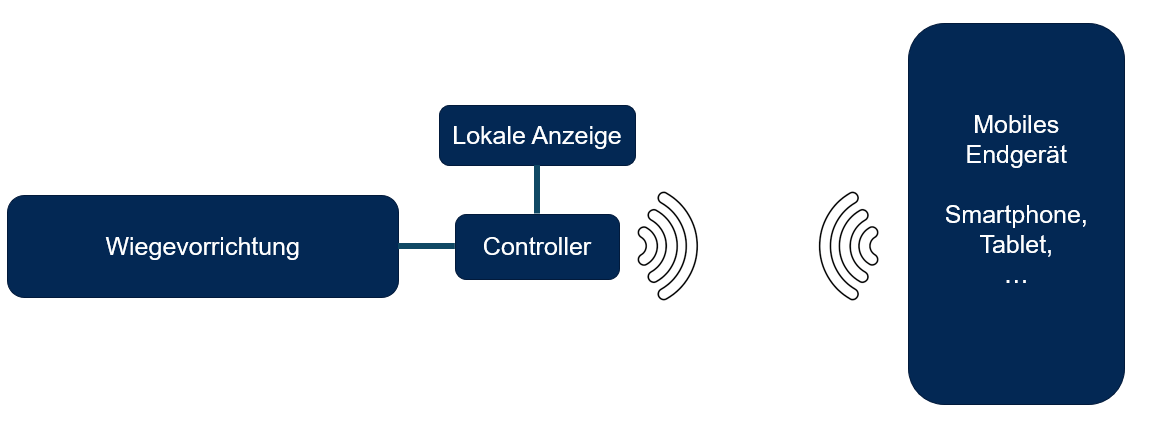
\includegraphics[width=1\textwidth]{Bilder/HW-Aufbau.png}
	\caption{Aufbau der smarten Küchenwaage}
	\label{fig.:HW-Aufbau}
\end{figure}
Da mit der Erstellung einer eigenen Küchenwaage die meisten Freiheiten und das größte Lern-Potential ist, wurde sich für diesen Weg entschieden. Der allgemeinen Systemaufbau ist in Abbildung \ref{fig.:HW-Aufbau} dargestellt. Um ein Objekt zu wiegen benötigt es eine zentrale Wiegevorrichtung, welche über einen Mikrocontroller angebunden ist, die lokale Anzeige des Gewichts übernimmt ein separates Bauteil. Über den Mikrocontroller selbst oder einem eigenständigen Bauteil soll die Kommunikation  mit einem mobilen Endgerät aufgebaut werden. 


\subsection{Controller}

Der Controller der smarten Waage sollte möglichst kostengünstig sein und einen geringen Stromverbrauch aufweisen um gegebenenfalls auch mit einer Batterie betrieben werden zu können. Aus diesem Hintergrund wird ebenfalls zur Kommunikation mit dem mobilen Endgerät \ac{BLE} verwendet. Bestehende Möglichkeiten für den Controller sind somit die Mikroprozessoren von Arduino oder RaspberryPi.
Da die Aufgabe der Prozessoren lediglich in der Messwerterfassung, Anzeige und Übertragung liegt, scheint der RaspberryPi überdimensioniert. In der Familie der Arduino-Mikroprozessoren sind die folgenden Boards mit Bluetooth ausgestattet: 
\begin{itemize}
	\item Nano IOT
	\item Nano BLE
	\item Nano BLE Sense
	\item BT
	\item Genuino 101
	\item MKR VIDOR 4000
\end{itemize}

Ebenso besteht die Möglichkeit ein eigenes Bluetooth-Modul wie das  HM10 BLE 4.0 anzuschließen, da nur ein sehr kompakter Bauraum vorhanden ist (siehe Kapitel \ref{Kap.:Wiegevorrichtung}), wird sich zur Auswahl auf die zuvor beschriebenen Boards beschränkt, im speziellen auf die kleinen Nano Boards. Da das Messen der Umgebung nicht gebraucht wird, entfällt der BLE Sense, eine finale Größe des Codes ist noch nicht vorhersehbar, weshalb sich für den Nano BLE entschieden wird, da dieser einen größeren Speicher besitzt. 


\subsection{Wiegevorrichtung\label{Kap.:Wiegevorrichtung}} 

Zur Aufnahme des Gewichts wird eine Wiegevorrichtung benötigt, diese setzt sich aus Sensor zur Messung des Gewichts, Standbein und Plattform für den zu messenden Gegenstand zusammen. 

Innerhalb der Wägetechnik werden oft Wäghezellen verwendet, diese bestehen aus einem Federkörper mit Dehnungsstreifen. Über diese kann ein analoges Signal erzeugt werden, welches auf die über der Wägezelle abgeleiteten Masse schließen lässt. Mittels eines Digital Analog Konverters, im speziellem dem HX711, kann ein digitales Signal erzeugt werden und an den Arduino zur Weiterverarbeitung gesendet werden.

Die Wägezelle selbst ähnelt einem Quader, welcher über eine Seite mit einem Fuß und auf der anderen mit der Plattform befestigt wird. Um das Messen komfortabel zu gestalten, wurden zwei baugleiche Teile entworfen und mithilfe von einem 3D-Drucker erzeugt. Die Entwürfe der Teile sind in Abbildung \ref{fig.:3D-Druck} dargestellt.

\begin{figure}[hbtp]
	\centering
	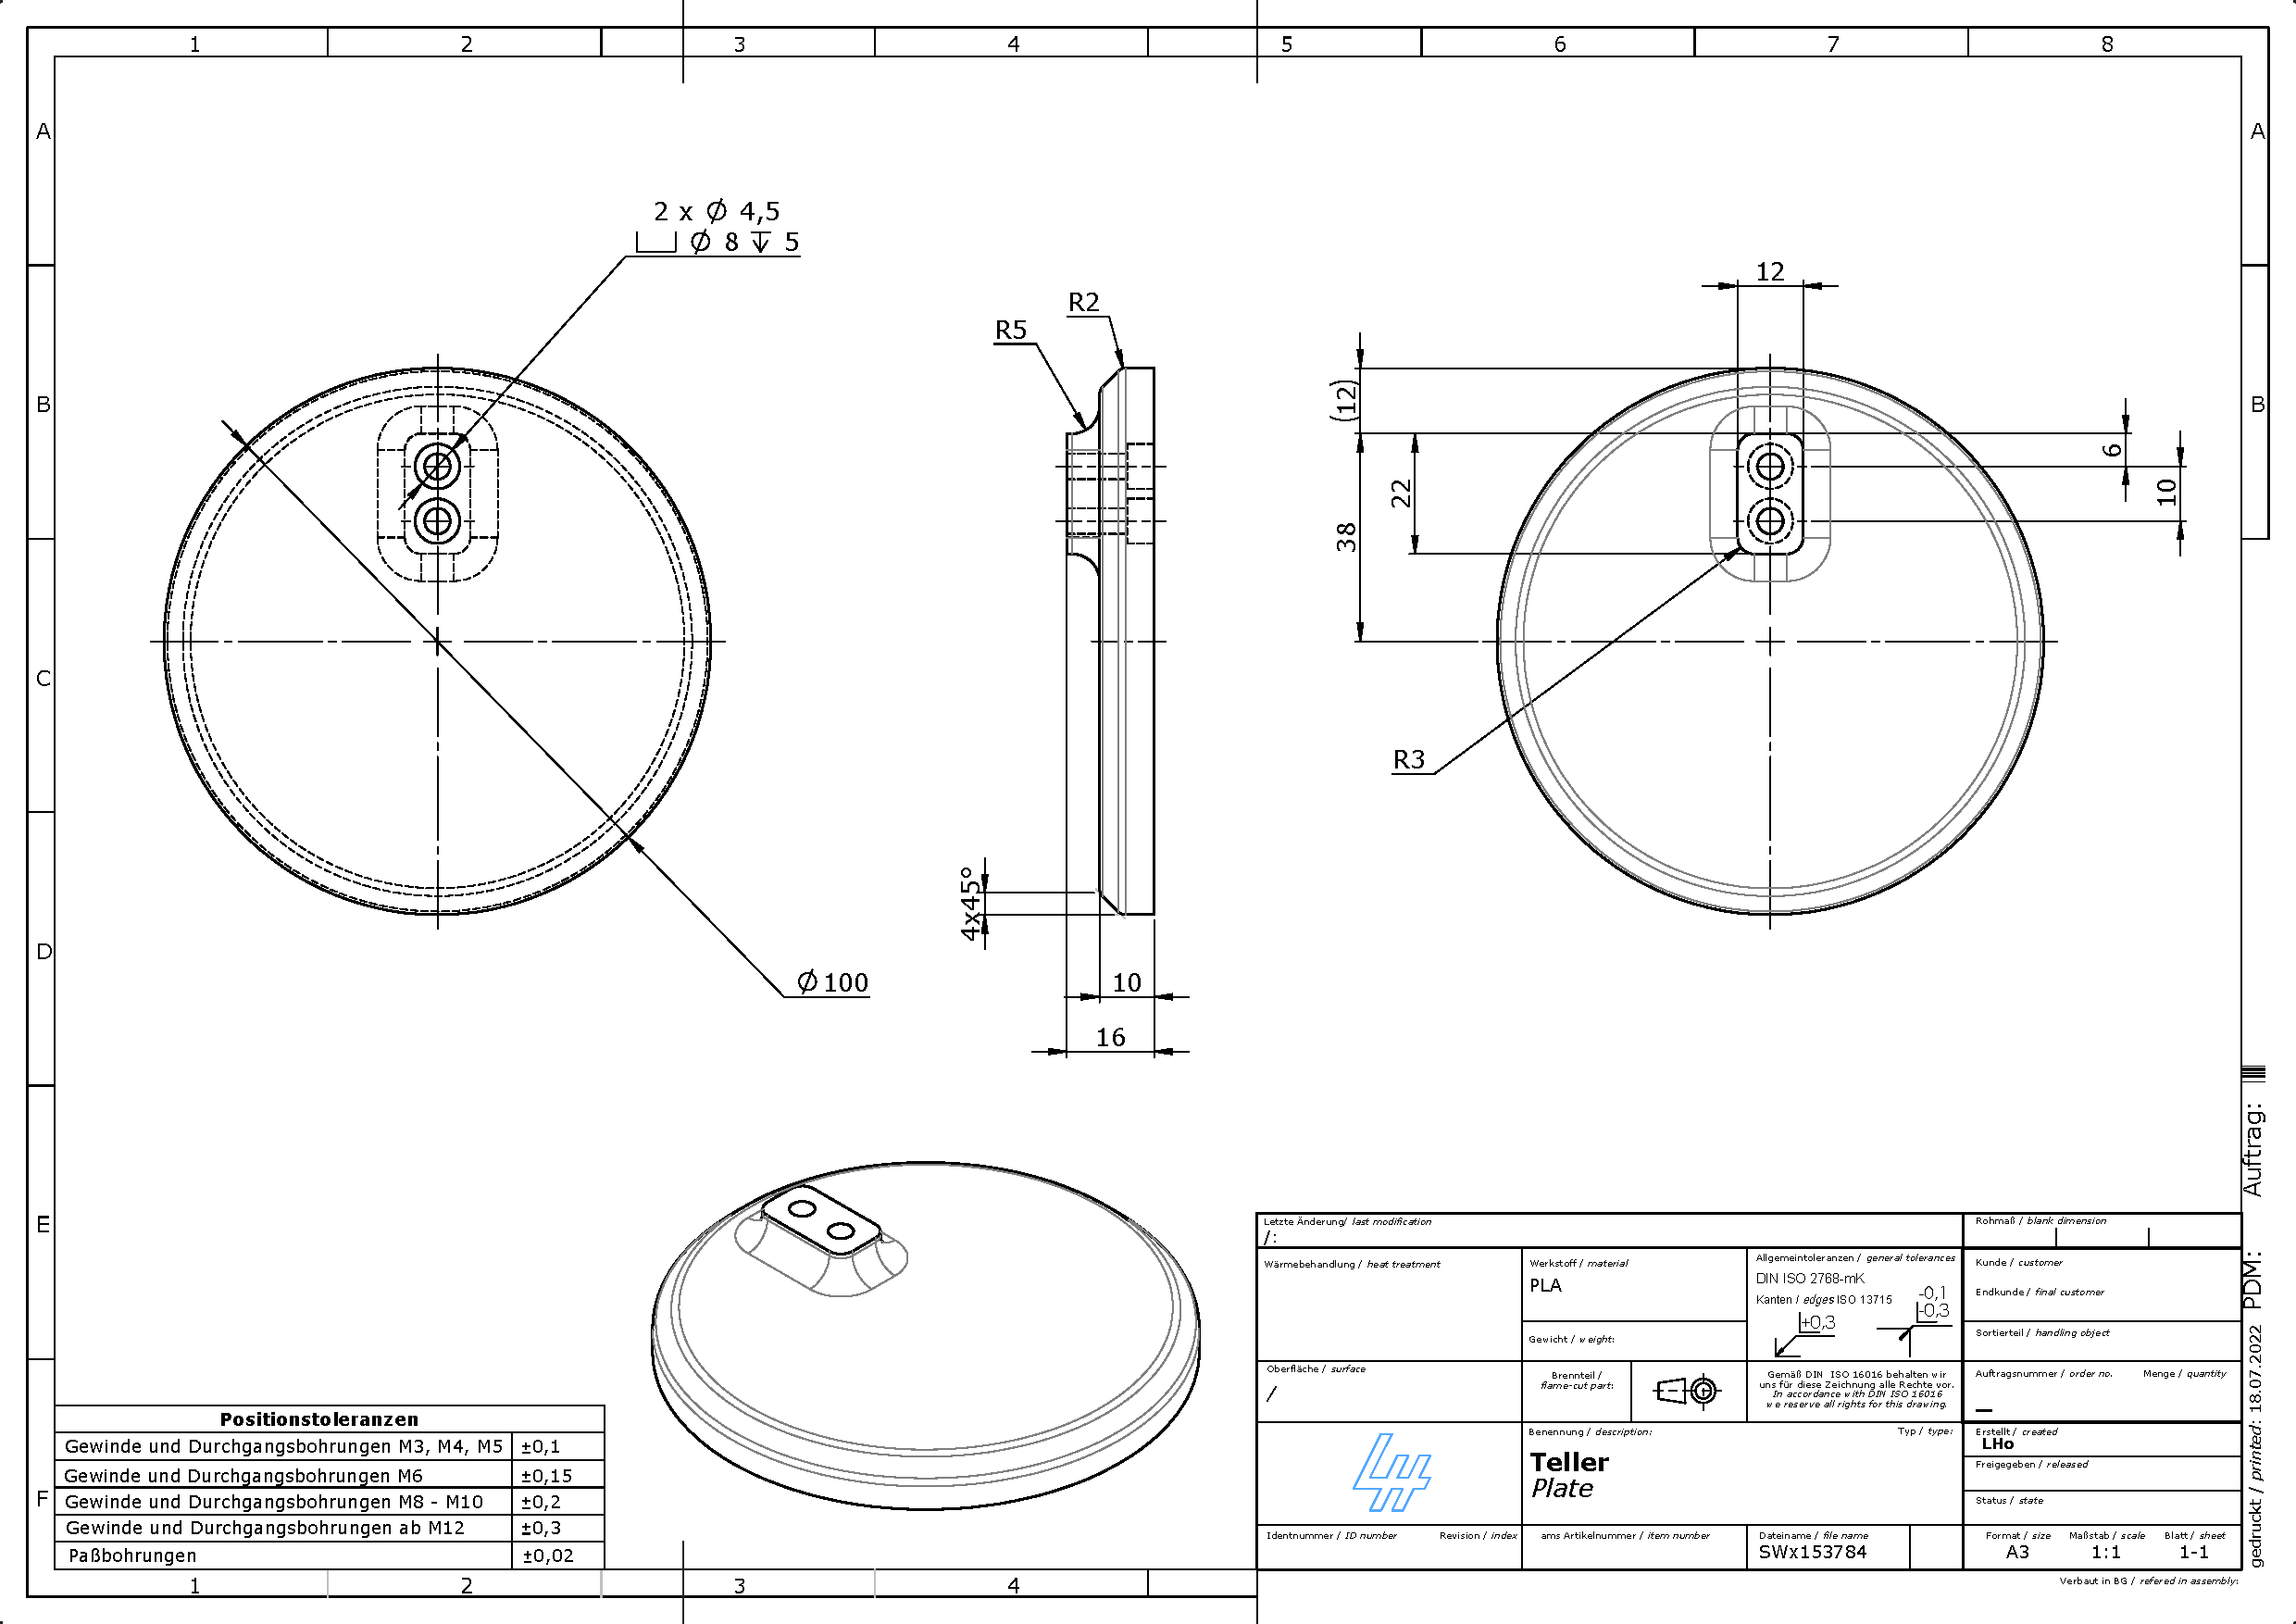
\includegraphics[width=1\textwidth]{Bilder/Teller-1.pdf}
	\caption{Entwurf des Fußes und der Wägeplattform der Waage}
	\label{fig.:3D-Druck}
\end{figure} 

Die Erhöhung ist nötig, um der Wägezelle zum messen genügend Spiel einzuräumen. Das Bauteil wird zweimal gedruckt und horizontal, sowie vertikal um 180 Grad entgegengesetzt an der Zelle angebracht, zu sehen in Abildung \ref{fig.:System}.

\begin{figure}[hbtp]
	\centering
	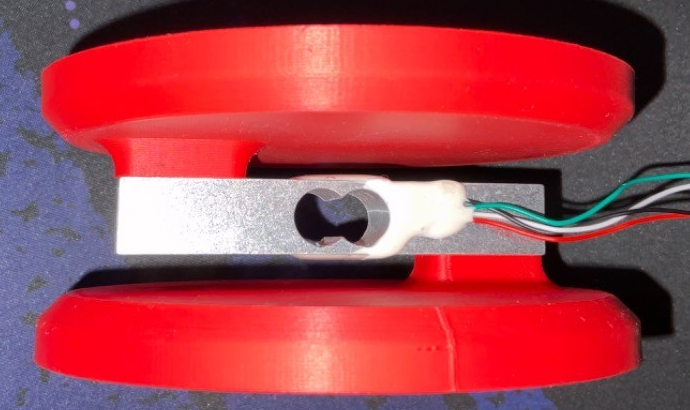
\includegraphics[width=1\textwidth]{Bilder/System.png}
	\caption{Die 3D gedruckten Teile sind mit M4-Schrauben an der Wägezelle befestigt, hierzu wurde eine Aussparung an der Unterseite der Teile für die Schrauben gelassen.}
	\label{fig.:System}
\end{figure} 

\subsection{lokale Anzeige}

Um die Küchenwaage auch ohne mobilem Endgerät nutzen zu können, wird eine Anzeige des aktuellen Gewichts benötigt, die Wägezelle hat ein Maximalgewicht von 10 kg, da beim Backen oder Kochen die Menge der Zutaten teilweise sehr genau bestimmt werden muss, sollte die Anzeige mindestens 4 stellen besitzen um bis auf 9999 g grammgenau wägen zu können. Um die Hardwarekosten sowie den Stromverbrauch der Waage möglichst gering zu halten, wird eine 7 Segmentanzeige mit 4 Stellen verbaut.  

\subsection{Verbinden der Komponenten}

Die soeben vorgestellten Komponenten müssen nun mit dem Controller verbunden werden. Für die prototypische Umsetzung wird mithilfe eines Steckbretts gearbeitet, in einem finalen Produkt kann der 3D-Druck jedoch so angepasst werden, dass die Komponenten zwischen Fuß und Messvorrichtung untergebracht und verkleidet werden. Die physische Verbindung der Komponenten ist in Abbildung \ref{fig.:Frizzing} zu sehen.

\begin{figure}[hbtp]
	\centering
	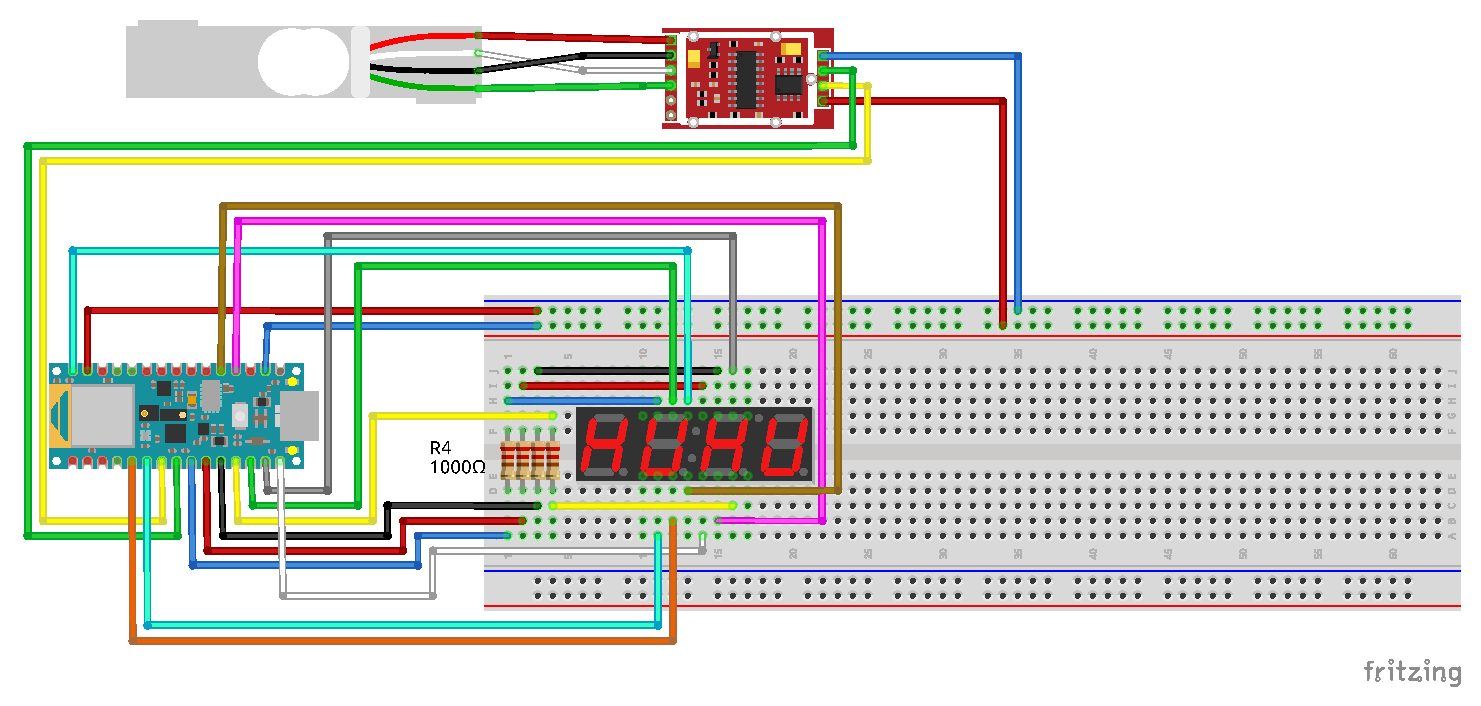
\includegraphics[width=1\textwidth]{Bilder/Platinenlayout.pdf}
	\caption{Die Komponenten sind mit dem Arduino verbunden, sollte im Folgenden Kapitel \ref{Kap.:Software} auf Pins eingegangen werden, entspricht dies der hier abgebildeten Verkabelung.}
	\label{fig.:Frizzing}
\end{figure} 

\section{Software\label{Kap.:Software}}

Mit dem Zusammenstellen der Komponenten wird nun die passende Software benötigt, diese teilt sich auf in Software für den Microcontroller und für das mobile Endgerät.

\subsection{Arduino}
Essentiell für den Erfolg des Projektes ist die Datenerfassung, Datenvorverarbeitung und Datenübertragung vom Microcontroller, da verschiedene Hardwarekomponenten verwendet werden, wird der Programmcode seperat beschrieben und anschließend zu einem Sketch zusammengeführt. 

\subsubsection{Wägezelle}

Die Wägezelle ist wie bereits beschrien mit einem Digital Analog Converter verbunden, dieser wird neben der Spannungsversorung über 3,3 V und Ground mit zwei digitalen Pins des Arduions verbunden, wobei einer der Pins zur Regelung des Taktes und die andere zur Signalübertragung genutzt wird. Z

um Auslesen des Sensors wird die Bibliothek HX711.h verwendet. 
Nach dem initialen tarieren der Waage mit einem bekannten Gewicht, was idealerweise 50\% des zulässigen Gesamtgewichts der Waage schwer ist, kann das aktuelle Gewicht mit nur einem Funktionsaufruf bestimmt werden. Um nicht 
\subsubsection{BLE\label{Kap.:BLE}}
\subsubsection{Segmentdisplay}
\subsection{App}
\subsubsection{Framework}
\subsubsection{BLE}
\subsubsection{Frontend}
\section{Zusammenfassung und Ausblick \label{Kap.:Zusammenfassung}}
\subsection{Reflexion}% (Takt-, BLE-, … Probleme)
\subsection{Ausblick} %(bessere Teller für die Waage, smartes Kochbuch, Foodtacker, Social Funktionen, …)

\section{Einführung}

Bei diesem Dokument handelt es sich um eine \LaTeX\ Vorlage für wissenschaftliche Arbeiten in der \ac{FEIF}. Es handelt sich hierbei nicht um eine Anleitung wie \LaTeX\ funktioniert, sondern rein um eine Vorlage die den formalen Richtlinien der \ac{FEIF} entspricht.

Es werden lediglich Hinweise und Tipps für das Arbeiten mit \LaTeX\ gegeben, so dass das arbeiten mit dieser Vorlage erleichtert wird. Anleitungen und Tutorials wie \LaTeX\ grundsätzlich funktioniert und die Syntax aufgebaut sind zu genüge im Internet vorhanden.

Eine gute Quelle hierfür ist die Dokumentation von \enquote{Overleaf} \footnote{\url{https://www.overleaf.com/learn}} oder das \enquote{Kochbuch für \LaTeX} \footnote{\url{https://archiv.dante.de/TeX-Service/TSP/tex/cookbook/cookbook.html}}. Eine weitere Hilfestellung ist es, die \LaTeX\ Datei dieses Dokuments zu öffnen um die verwendeten Syntax für die Erstellung zu sehen. Diese steckt voller nützlicher Beispiele wie mit dieser Vorlage Effizient gearbeitet werden kann.

\section{Entwicklungsumgebung}

Zunächst lohnt es sich, eine passende \ac{IDE} zu wählen. Hier gilt es, sich zwischen einer Online oder Offline Entwicklungsumgebung zu entscheiden.

\subsection{Online Entwicklungsumgebung}

Soll eine Online \ac{IDE} gewählt werden so empfiehlt sich die Verwendung von \enquote{Overleaf} \footnote{\url{https://www.overleaf.com}}. Diese läuft rein browserbasiert und ermöglicht das gemeinsame Arbeiten an einem Dokument. Um es zu nutzen muss man sich lediglich mit einer E-Mail-Adresse anmelden.

\subsection{Offline Entwicklungsumgebung}

Bei einer Offline \ac{IDE} handelt es sich um ein Programm, was auf dem Rechner installiert werden muss. Auch für die Installation von \LaTeX\ gibt es im Internet viele Anleitungen. Eine Programmempfehlung wäre das kostenfreie Programm \enquote{TEXMAKER} \footnote{\url{https://www.xm1math.net/texmaker/}}. Hierbei handelt es sich um eine Entwicklungsumgebung, die unter den Betriebssystemen Linux, MacOS und Windows funktioniert. Sie ist flexibel nach den eigenen Wünschen anpassbar, bietet eine Vielzahl von Assistenzfunktionen, eine gute Syntax-Highlighting Funktion und eine integrierte Dokumentenvorschau.

Natürlich können auch andere Programme verwendet werden, auch hier führt eine Internetrecherche zu vielen Ergebnissen.

\section{Funktionalitäten}

In diesem Kapitel wird auf die Funktionalitäten dieser Vorlage eingegangen. Vielen erscheint \LaTeX\ Anfangs sehr kompliziert, da es sich dabei um eine Skriptsprache handelt, die nicht wie klassische Textverarbeitungsprogramme auf das \enquote{\ac{WYSIWYG}} Prinzip setzt. So wird hier der Inhalt und die Formatierung erst nach dem übersetzten des Codes sichtbar. Dies erscheint für viele auf den ersten Blick ein Nachteil und Behinderung zu sein, jedoch ist das Gegenteil der Fall. Im Folgenden wird auf nützliche Funktionalitäten eingegangen, die einem nicht jedes Textverarbeitungsprogramm zur Verfügung stellt.

Im folgenden werden die Funktionalitäten beschrieben, jedoch auch hier der Hinweis: Es gibt keine expliziten Codebeispiele im Text, die verwendeten \LaTeX\-Befehle sind nur im Quellcode zu sehen.

\subsection{Verzeichnisse}

Einer der größten Vorteile ist es, dass Verzeichnisse automatisch erstellt werden. Grundvoraussetzung ist hierbei lediglich, dass die richtigen Befehle an den entsprechenden Stellen verwendet werden.

\subsubsection{Inhalt}

Das Inhaltsverzeichnis wird durch die Verwendung von Überschriften im Text automatisch erstellt. Wird eine neue Überschrift hinzugefügt, taucht diese an der entsprechenden Stelle im Inhaltsverzeichnis auf. Wird eine Überschrift gelöscht, so wird sie auch aus dem Inhaltsverzeichnis entfernt.

Die Gliederungstiefe in diesem Dokument ist dreistufig:

\begin{enumerate}
	\item Überschrift 1 (section)
	\begin{enumerate}
		\item Überschrift 1.1 (subsection)
		\begin{enumerate}
			\item Überschrift 1.1.1 (subsubsection)
		\end{enumerate}
	\end{enumerate}
\end{enumerate}

\subsection{Abbildungen}

Auch das Abbildungsverzeichnis wird automatisch erstellt, hierzu muss eine Abbildung mit entsprechender Syntax eingebunden werden. In diesem Beispiel haben wir in Abbildung \ref{fig: Logo der Hochschule Coburg} das Logo der Hochschule Coburg als Bild eingebunden. Ebenfalls wird die Position des Bildes und dessen Größe fest vorgegeben. 

\begin{figure}[hp]
	\centering
	
\includegraphics[width=1\textwidth]{Bilder/Titelseite/Logo_HS_Coburg}
	\caption{Logo der Hochschule Coburg}
	\label{fig: Logo der Hochschule Coburg}
\end{figure}

In Abbildung \ref{fig: Logo der Hochschule Coburg - kleiner dargestellt} ist das identische Bild aus Abbildung \ref{fig: Logo der Hochschule Coburg} dargestellt, lediglich verkleinert. Durch den \enquote{captiion} Befehl tauchen beide Abbildungen im Abbildungsverzeichnis mit entsprechendem Verweis auf die Seite im Dokument automatisch auf.

\begin{figure}[hp]
	\centering
	
\includegraphics[width=0.5\textwidth]{Bilder/Titelseite/Logo_HS_Coburg}
	\caption{Logo der Hochschule Coburg - kleiner dargestellt}
	\label{fig: Logo der Hochschule Coburg - kleiner dargestellt}
\end{figure}

\newpage

\subsection{Tabellen}

Tabellen mit \LaTeX\ zu erstellen ist zugegebenermaßen etwas umständlich, jedoch stellen viele Programme Assistenzfunktionen für das erstellen zur Verfügung. Wurde das Arbeiten mit Tabellen in \LaTeX\ verstanden, so stellt dies kein Problem mehr dar. Tabellen wie Tabelle \ref{tab: Beipsieltabelle} können so mit Leichtigkeit erstellt werden. Auch diese Tabelle taucht automatisch im Tabellenverzeichnis auf.

\begin{table}[hp]
	\begin{tabular}{| L{3cm} | l | l |}
	\hline
	\rowcolor{lightgray}
	Kopfzeile 1 mit fester Breite & Kopfzeile 2 mit dynamischer Breite & Kopfzeile 3 (dynamisch)\\
	\hline
	In dieser Tabellenzeile entsteht ein automatischer Zeilenumbruch wenn der Rand überschritten wird. & Hier nicht, sie wird dynamisch erweitert. & \cellcolor{blue} Ich bin blau.\\
	\hline
	Achtung, unter meiner Zelle fehlt die horizontale Trennlinie & \multicolumn{2}{r}{Zellenverbindung, rechtsbündig, ohne rechten vertikalen Rand}\\
	\cline{2-3}
	\multicolumn{3}{| c |}{Tabellenende}\\
	\hline
	\end{tabular}
\caption{Beispieltabelle}
\label{tab: Beipsieltabelle}
\end{table}

\subsection{Code}

Oft git es in der Elektrotechnik und Informatik Code zu dokumentieren. Auch hier bietet \LaTeX\ gute Möglichkeit. Es werden nahezu alle Programmiersprachen unterstützt, ebenfalls ist ein angepasstes Syntax-Highlighting möglich. Im Codebeispiel \ref{code: Beispielcode} ist eine for-Schleife in MATLAB realisiert. Auch dieses Beispiel taucht automatisch im Codebeispielverzeichnis auf.

\begin{lstlisting}[caption={Beispielcode MATLAB}, label=code: Beispielcode]
for v = 1.0:-0.2:0.0
   disp(v)
end
\end{lstlisting}

\subsection{Symbole}

Das Symbolverzeichnis dient der Darstellung von Symbolen, welche in Formeln verwendet werden. Hier ist darauf zu achten, dass die Symbole in der .tex-Datei \enquote{Symbolverzeichnis.tex} im Ordner \enquote{Dateien/Verzeichnisse/} eingetragen werden. Die dort eingetragenen Symbole werden automatisch alphabetisch geordnet und aufgelistet.

Auch hier wieder ein Beispiel:

\begin{equation}
	\overline{x} = \frac{1}{n} \sum_{i=1}^n x_i
\end{equation}

\begin{equation}\label{term: Formel}
	s = \sqrt{\frac{1}{n - 1} \sum_{i=1}^n (x_i - \overline{x})}
\end{equation}

Hier werden die Formeln automatisch nummeriert, ebenfalls kann auf diese Nummerierung eine Referenzierung erfolgen (siehe Formel \ref{term: Formel}).

\subsection{Abkürzungsverzeichnis}

Abkürzungen wurden schon im Laufe des Dokumentes verwendet. Auch hier gilt die Abkürzungen in der Datei \enquote{Abkuerzungsverzeichnis.tex} im Order \enquote{Dateien/Verzeichnisse/} auszufüllen. Das Verzeichnis wird automatisch erstellt und alphabetisch geordnet ausgegeben. Bei erstmaliger Verwendung wird die Abkürzung automatisch ausgeschrieben und steht dahinter in Klammern. Allerdings gibt es verschiedene Möglichkeiten, Abkürzungen auszugeben.

\begin{itemize}
	\item acs: \acs{EBA}
	\begin{itemize}
		\item Auch wenn die Abkürzung neu ist gibt dieser Befehl nur die Abkürzung aus.
	\end{itemize}
	\item ac: \ac{EBA}
	\item acl: \acl{EBA}
	\begin{itemize}
		\item Hier wird eine vollständige Ausgabe der Abkürzung erzwungen.
	\end{itemize}
\end{itemize}

\subsection{Glossar}

Auch für die Erstellung des \gls{Glossar}s gibt es eine einfache Möglichkeit. Die Begriffe, welche im \gls{Glossar} auftauchen sollen müssen in der Datei \enquote{Glossar.tex} im Ordner \enquote{Dateien/Verzeichnisse/} eingetragen werden. Dort eingetragene Begriffe können mit den entsprechenden Befehlen im Text aufgeführt werden. Wurden Begriffe in der Glossar Datei angelegt, allerdings nicht im Dokument verwendet, erscheinen diese bei der Ausgabe nicht im \gls{Glossar}s. Die Ausgabe des \gls{Glossar} erfolgt alphabetisch geordnet.

\underline{\textbf{Hinweis}}

Für das erstellen des Glossars kann es notwendig sein, den Befehl \enquote{makeglossaries} auszuführen.

\subsection{Literatuverzeichnis}

Das Literaturverzeichnis wird mit Hilfe von BibTex erstellt. Hierzu muss die verwendete Literatur in der Datei \enquote{Literatur.bib} im Ordern \enquote{Literatur/} eingetragen werden.

Hier noch Beispiele für das Zitieren mit \LaTeX\ :

\enquote{The engineers started trying to understand how heat would dissipate and current flow would behave across seventy batteries by supergluing them together into groups called bricks.} \cite[S. 158]{Vance2016}

Eine Faltung zweier Funktionen im Zeitbereich gestaltet sich als kompliziert, eine Vereinfachung bringt es, die Funktionen in den Laplace-Bildbereich zu überführen. Die Faltung im Zeitbereich entspricht einer Multiplikation im Bildbereich. \cite[S. 339f]{Papula2006}























 

%	---------------------------------	%
%		Literaturverzeichnis				%
%	---------------------------------	%

% Literaturverzeichnis soll im Inhaltsverzeichnis auftauchen
\newpage
\addcontentsline{toc}{section}{Literaturverzeichnis}

% Literaturverzeichnis anzeigen
\renewcommand\refname{Literaturverzeichnis}
\bibliography{Literatur/Literatur}


%	---------------------------------	%
%			 Glossar					%
%	---------------------------------	%

% Glossar ausgeben
\newpage
%\renewcommand*{\glspostdescription}

% alle Einträge im Glossar ausgeben
%\setglossarystyle{altlist}
%\glsaddall % alle Einträge, egal ob verwendet oder nicht verwendet anzeigen
%\printglossary
%\newglossaryentry{Glossar}
{
    name=Glossar,
    plural=Glossare,
    description={\enquote{selbstständig oder als Anhang eines bestimmten Textes erscheinendes Wörterverzeichnis} \cite{Duden}}
}


%	---------------------------------	%
%			 	Anhang					%
%	---------------------------------	%

\newpage
\fancyhead[L]{Anhang} %Kopfzeile links
\appendix



%	---------------------------------	%
%		Ehrenwörtliche Erklärung			%
%	---------------------------------	%

\newpage
\addcontentsline{toc}{section}{Ehrenwörtliche Erklärung}
\fancyhead[L]{Ehrenwörtliche Erklärung} %Kopfzeile links
\begin{centering}
\textbf{{\huge Ehrenwörtliche Erklärung}}
\par
\end{centering}

\vspace{2cm}

Ich versichere hiermit, dass ich meine/n Praxisbericht/Bachelorarbeit/Masterarbeit mit dem Titel

\vspace{2cm}

\begin{tabular*}{\linewidth}{@{\extracolsep{\fill}}ccc}
 \\ \hline
 \vspace{2cm}
 \\ \hline
\end{tabular*}

\vspace{2cm}

selbständig verfasst, keine anderen als die angegebenen Quellen und Hilfsmittel benutzt sowie nicht an anderer Stelle als Prüfungsarbeit vorgelegt habe.

\vfill

\begin{tabular*}{ccc}
\cline{1-1}
\parbox{7cm}{\raggedright Ort} &
\parbox{3cm}{\raggedright} &
\parbox{7cm}{\raggedright} \\
\vspace{2.5cm} \\
\cline{1-1} \cline{3-3}
\parbox{7cm}{\raggedright Datum} &
\parbox{3cm}{\raggedright} &
\parbox{7cm}{\raggedright Unterschrift} \\ 
\end{tabular*}



\end{document}